\chapter{Machine Learning Basics}\label{chap:basics}

This chapter presents basic concepts and definitions about machine learning, including data representation, dataset, hypothesis space, inductive bias, and various learning tasks and learning schemes. Moreover, we will also discuss density estimation, ground truth, and underlying data distribution.

\subsection*{What is machine learning?} 

A machine learning algorithm is a software program that can improve its performance by learning from data (or examples).  As shown in Figure~\ref{fig:learning}, given a program (or model) $f$, the improvement (from $f$ to $f'$) is achieved by applying a learning algorithm on $f$ and a set $D_{train}$ of training instances.  

\begin{figure}[!htbp]
    \centering
    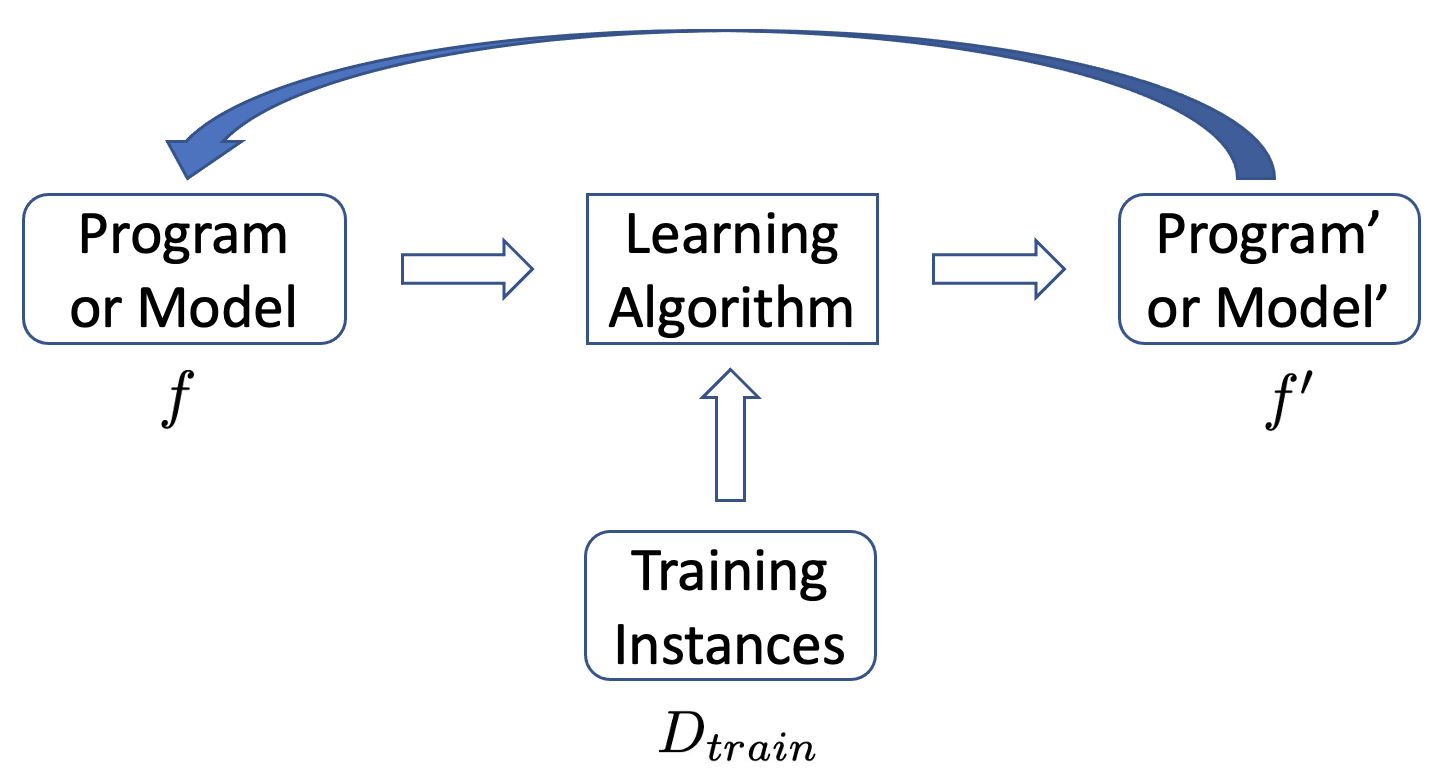
\includegraphics[width=0.7\textwidth]{images/foundations/learning.png}
    \caption{Machine learning}
    \label{fig:learning}
\end{figure}

Usually, a learning algorithm cannot fully comprehend the training instances with a single pass. Therefore, the learning over a dataset $D_{train}$ is an iterative process, i.e., the learning step shown in Figure~\ref{fig:learning} is repeated until a termination condition is satisfied. A termination condition can be e.g., a number of iterations, an accuracy threshold, and a convergence condition. 

Based on the above process, and depending on the nature of the data instances and how the learning algorithm interacts with the data instances, there can be different learning tasks and learning schemes. We will briefly discuss the basic categories of them in Section~\ref{sec:learningtasks} and Section~\ref{sec:learningschemes}, leaving the details of the learning algorithms to 
Part \ref{chap:simple} and Part \ref{chap:deep}. In the following, we explain the data representation (Section~\ref{sec:datarep}) and the datasets (Section~\ref{sec:datasets}). 


\section{Data Representation}

Data representation refers to the way how the data instances are stored and represented. A suitable data representation can ease the storage, transmission, and processing of data, and more importantly, benefit the machine learning algorithms which heavily rely on not only the data but also the way how the data is operated.  

\subsection*{Representing instances using feature vectors}\label{sec:datarep}

A dataset is formed of a finite set of data instances as well as their associated labels if available. One common way to represent a data instance is to use a fixed-length vector $\textbf{x}$ to represent the features (or attributes) of the data instance. 
%
Standard feature types include e.g., 
\begin{itemize}
    \item nominal (including Boolean) type, such that there is no ordering among possible values of the feature. For example, $color \in \{red, blue, green\} $ is a nominal feature. 
    \item ordinal type, such that possible values of the feature are totally ordered. For example, $size \in \{small, medium, large\} $ is an ordinal type. 
    \item numeric (continuous) type, whose values are stored as groupings of bits, such as bytes and words. Numbers, such as integers and real numbers, are typical examples of numeric types. As an example, $weight \in [0...500]$ is a numeric type. 
    %\item hierarchical, where possible values are partially ordered in a hierarchy. 

\end{itemize}

\begin{example}\label{example:iris}
For the \textbf{iris} dataset \cite{Dua:2019}, we have the information in Figure~\ref{fig:irisflowerexample} and Table~\ref{tab:irisdataset}. The left picture (Figure~\ref{fig:irisflowerexample}) is an illustration of an iris flower, where we can see the intuitive meanings of four features: sepal length, sepal width, petal length, and petal width. The right table (Table~\ref{tab:irisdataset}) is a snapshot of the dataset, which has in total of 150 instances. We can see that, all four features are represented as numeric values. 
\begin{table}[!htbp]
\small
\begin{minipage}{0.35\textwidth}
    \centering
    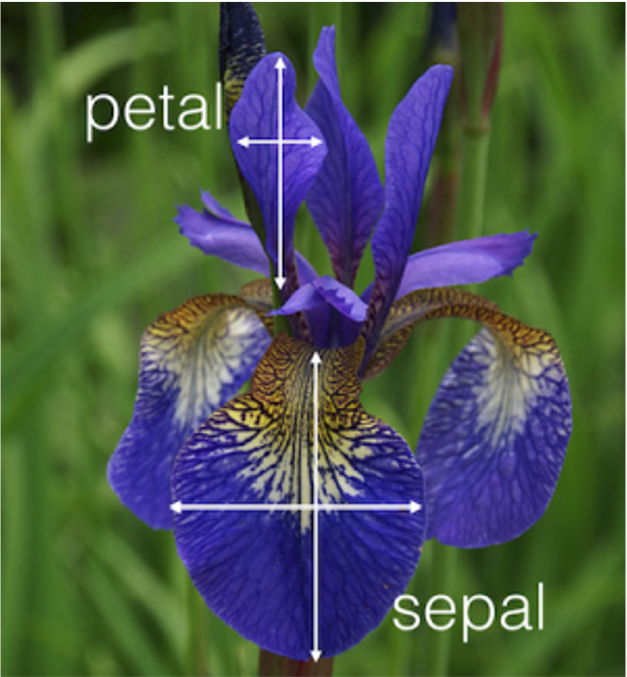
\includegraphics[width=\textwidth]{images/foundations/iris.png}
    \caption{An iris flower}
    \label{fig:irisflowerexample}
\end{minipage}~~~~~
\begin{minipage}{0.6\textwidth}
    \centering
    \begin{tabular}{|c|c|c|c|c|l|}
    \hline
       index  & Sepal & Sepal & Petal & Petal & Class Label\\
         & Length & Width & Length & Width &  \\
         \hline
       1  & 5.1 & 3.5 & 1.4 & 0.2 & iris setosa \\
       2  & 4.9 & 3.0 & 1.4 & 0.2 & iris setosa \\
       ... &&&&& \\
       50  & 6.4 & 3.5 & 4.5 & 1.2 & iris versicolor \\
       ... &&&&&\\
       150  & 5.9 & 3.0 & 5.1 & 1.8 & iris virginica \\
       \hline
    \end{tabular}
    \caption{Iris dataset}
    \label{tab:irisdataset}
\end{minipage}
\end{table}
\end{example}


We may write $\textbf{x}=(x_1,...,x_n)$ for an instance with $n$ features, each of which has value $x_i$ for $i\in \{1,...,n\}$. 
%
Then, in case we are dealing with labelled data, we also need to represent the label of each instance $\textbf{x}$. Depending on the nature of the problem, a label can be represented as either a scalar $y$ (e.g., classification) or a vector $\textbf{y}$ (e.g., object detection). There are also tasks in which each label is a structured object. 

\begin{example}
For the \textbf{iris} example, we can see from Table~\ref{tab:irisdataset} that each instance is associated with a label indicating it is in one class (3 classes in total). If we use 1 for iris setosa, 2 for iris versicoler, and 3 for iris virginica, we may have $\textbf{x}_1=(5.1,3.5,1.4,0.2)$, and $y_1=1$. 
\end{example}

\begin{example}
In the \emph{object detection} task, a label is a set of bounding boxes, each of which is associated with not only a classification label but also other information such as the size of the box, the coordinates of the box in the image, etc. 
\end{example}
 
%After representing features of $x$ as a fixed-length vector, we also need to represent the label of each instance $y$. 

In the following, we may also write $(\textbf{x},y)$ for an instance, assuming that the label is a scalar number $y$. 

\subsection*{Feature space} 

We can think of each instance $\textbf{x}$ as representing a point in a $n$-dimensional feature space where $n$ is the number of features of $\textbf{x}$. 

\begin{example}\label{example:3dscatter}
Assume that we are working with a dataset which is sampled from the following underlying function: 
\begin{equation}
\begin{array}{rcl}
    X & \in & [0,7] \\
    Y & = & \sin{7X} + \epsilon \\
    Z & = & \cos{7X} + \epsilon \\
    \epsilon & \in & [0,1] 
\end{array}
\end{equation}
such that all instances contain 3 numerical features $X,Y,Z$. $\epsilon$ denotes the noise.  Each data instance  is a point in a 3-dimensional space. The visualisation of the dataset is seen in Figure~\ref{fig:3dscatter}. The code for the generation of the figure is given in Chapter~\ref{sec:foundationspracticals}. 

\begin{figure}[!htbp]
    \centering
    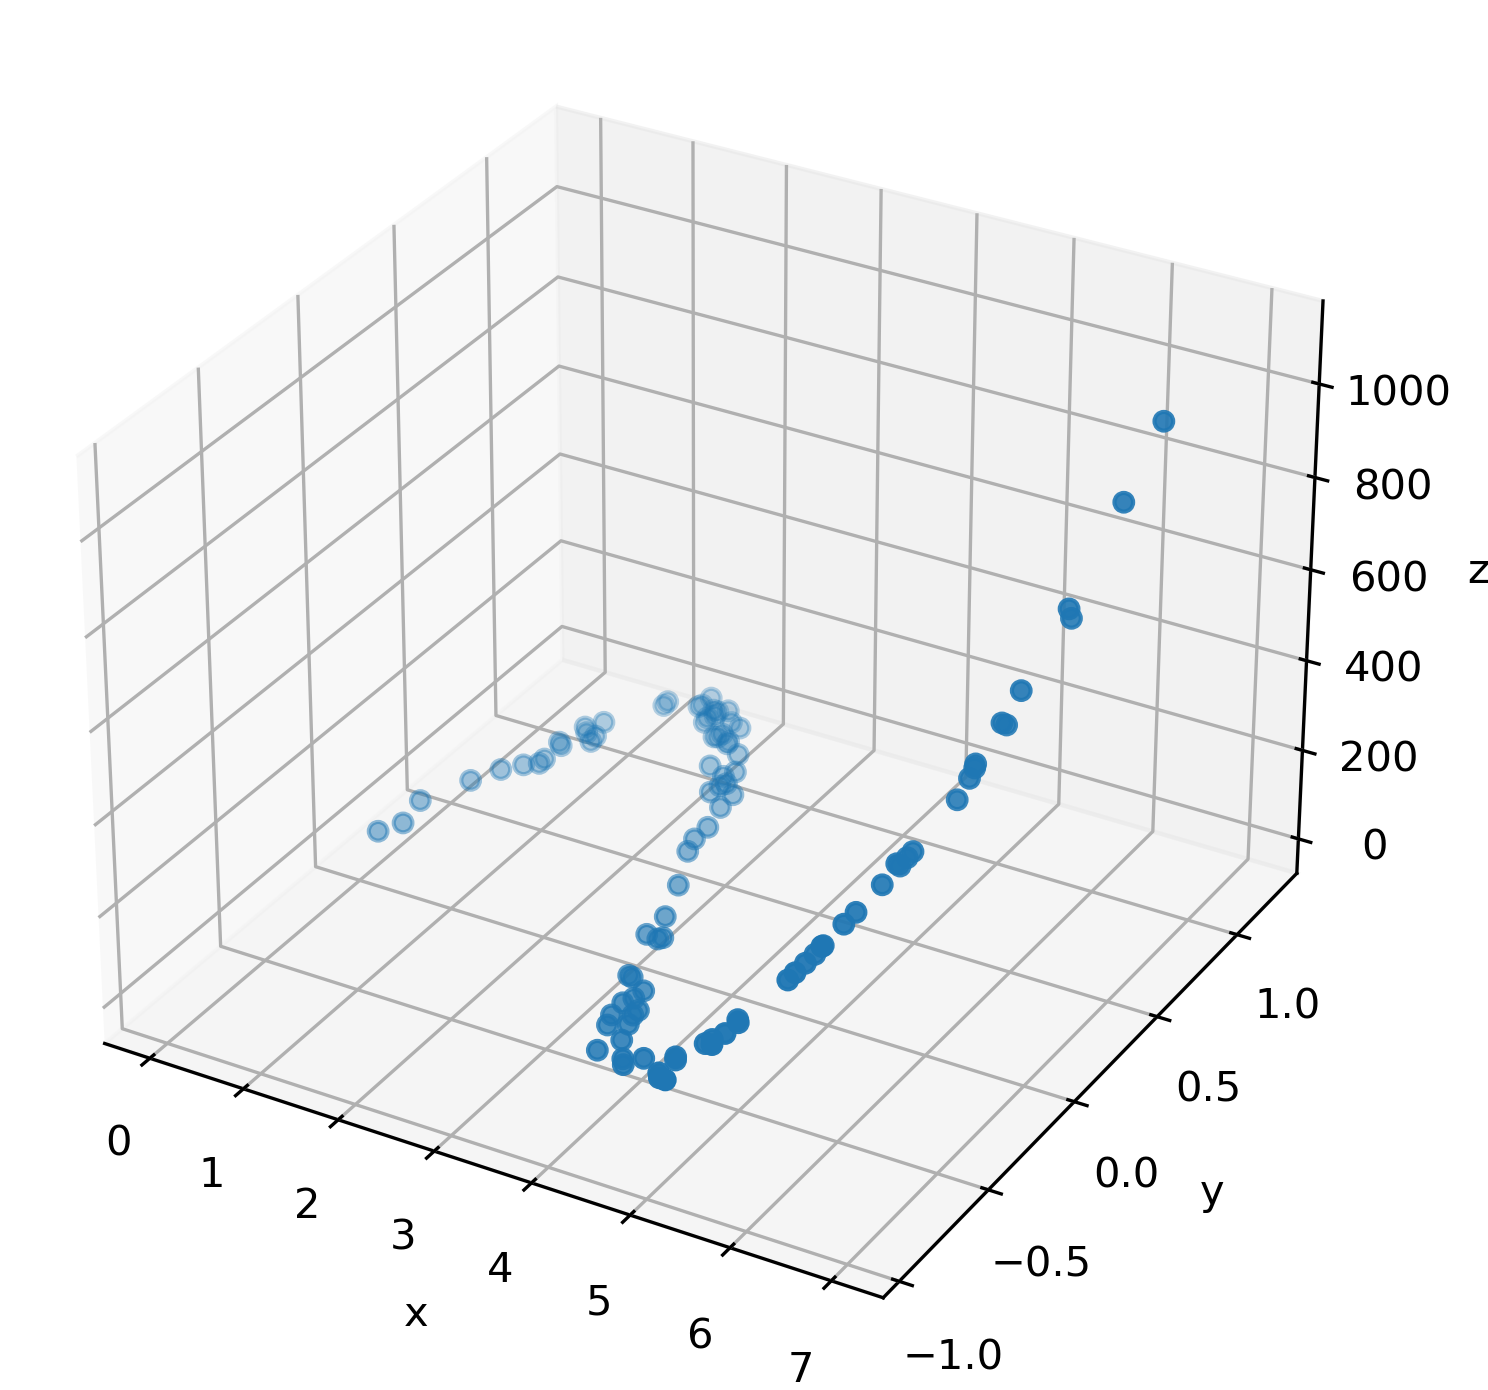
\includegraphics[width=0.6\textwidth]{images/foundations/3d_scatter.png}
    \caption{Visualisation of a 3-dimensional dataset}
    \label{fig:3dscatter}
\end{figure}
\end{example}

Assume that all features are numeric and every feature $X_i$ is in a set $R_i$. Then, the feature space is $\displaystyle \prod_{i=1}^n R_i = R_1\times ... \times R_n$.

\section{Datasets}\label{sec:datasets}

A dataset is a collection of data instances. According to their different roles in the machine learning lifecycle, we may have multiple datasets, including training dataset, test dataset, and validation dataset. 

\subsection*{Independent and identically distributed (i.i.d.) assumption}

We often assume that training instances are independent and identically distributed (i.i.d.), i.e., the instances are sampled from the same probability distribution (i.e., identically distributed) and all of them are mutually independent.
i.i.d. assumption has an important property for a valid dataset, because it enables the following property: 
\begin{tcolorbox}
the larger the size of the dataset becomes, the greater the probability of the data instances will closely resemble the underlying distribution. 
\end{tcolorbox} 
We remark that, this property is key to many machine learning theoretical results
%, which are 
based on e.g., Chebyshev's inequality, and Hoeffding's lemma.  

However, there are also cases where this assumption does not hold, such as 
\begin{itemize}
    %\item cases where the sets of instances have dependencies
    \item instances sampled from the same medical image,
    \item instances from time series,
    \item etc. 

\end{itemize}
For non-i.i.d. datasets, dedicated techniques have to be taken to make sure the learning algorithm can learn useful information instead of biased information.  

\subsection*{Training, test, and validation datasets}

The collected dataset can be split into two datasets, one for training and the other for test. We call them \emph{training dataset} and \emph{test dataset}, respectively.  The split does not have a fixed percentage, with e.g., 7:3 or 8:2 split being very commonly seen in practice.  Within the training dataset, there might be a subset called \emph{validation dataset} that is often used to control the learning process, such as the termination of the learning process or the selection of the learning directions and hyper-parameters. Figure~\ref{fig:dataset-split} presents an illustrative diagram for the three datasets. 

\begin{figure}[!htbp]
    \centering
    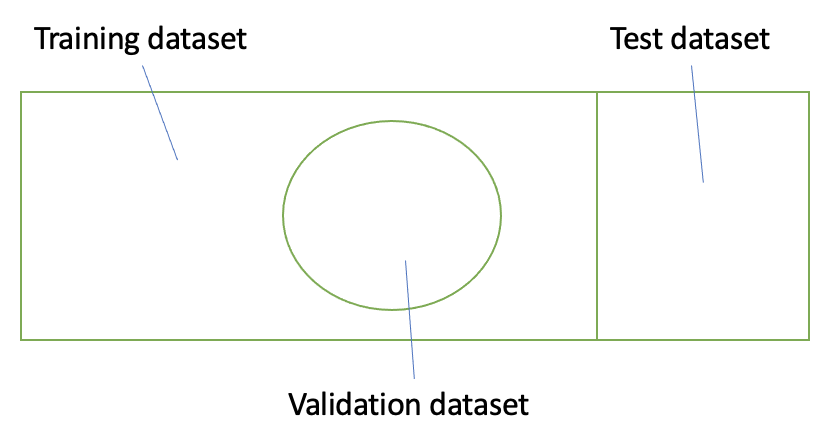
\includegraphics[width=0.5\textwidth]{images/foundations/dataset_split.png}
    \caption{Training, test, and validation datasets}
    \label{fig:dataset-split}
\end{figure}

\section{Hypothesis Space and Inductive Bias}

As suggested in Figure~\ref{fig:learning}, a learning agent $f$ is a program or model or function. It updates itself by learning from training data. Nevertheless, 
the function $f$ has to be chosen from a function space ${\cal H}$, called hypothesis space. Normally, the hypothesis space is determined by the learning algorithm. 

\begin{example}
For a decision tree algorithm, the hypothesis space is the set of all possible trees such that each tree node represents a feature and the branches of a tree node represent the split of the possible feature values. 
\end{example}

\begin{example}
For a linear regression algorithm, the hypothesis space is the set of linear functions $y=\textbf{w}^T\textbf{x}+b$, where $\textbf{w}\in \real^{|\textbf{x}|}$ and $b\in \real$. 
\end{example}

\begin{example}
For a neural network whose corresponding  function $f_{\textbf{W}}$ is parameterised over learnable weights $\textbf{W}$, the hypothesis space is the set of functions $f_{\textbf{W}}$ such that each weight in $\textbf{W}$ is a real number. 
\end{example}

The inductive bias (also known as learning bias) of a learning algorithm is the set of assumptions that the designer imposes on the hypotheses in ${\cal H}$ to guide the learner in its learning. Usually, the assumptions can be e.g., 
\begin{itemize}
    \item restrictive assumption that limits the hypothesis space, or 
    \item preference assumption that imposes ordering on hypothesis space, etc. 
\end{itemize}

\begin{example}
For decision tree learning, it is possible to ask for a preference over simpler trees, by following Occam's razor. 
\end{example} 

\begin{example}
For neural networks, it is possible to apply regularisation techniques, such as $L_1$ or $L_2$ regularisation, so that the learning algorithm will have a preference between weight matrices $\textbf{W}$ embedded. 
\end{example} 

 
\section{Learning Tasks}\label{sec:learningtasks}

Given a dataset, we also need to determine the learning task before applying machine learning algorithms. Different machine learning algorithms (and probably datasets) will be needed, according to different learning tasks.

\subsection*{Supervised learning}

One of the most frequently seen tasks is supervised learning, which learns a function according to a set of input-output pairs. The primary objective in supervised learning is to make sure that the learned function generalises, i.e., it is able to accurately predict label $y$ for previously unseen $\textbf{x}$.  

\begin{definition}
(Supervised Learning) Given a training set of instances sampled from an unknown target function $h$, i.e.,  
\begin{equation}
    D = \{(\textbf{x}^{(1)},y^{(1)}), (\textbf{x}^{(2)},y^{(2)}), ..., (\textbf{x}^{(m)},y^{(m)}) \}
\end{equation}
it is to learn a function $f\in {\cal H}$ that approximates the target function $h$, where ${\cal H}$ is a set of models (a.k.a. hypotheses). We call $D$ a labelled dataset when each instance $\textbf{x}$ is attached with a label $y$, and unlabelled, otherwise. 
\end{definition}

In the above definition, when $y$ is discrete, it is a \emph{classification} task (or concept learning). When $y$ is continuous, it is a \emph{regression} task. The function $f$ is called classifier or regressor, depending on the tasks. For a classifier, it is often that, instead of directly returning  a label,  $f(\textbf{x})$ returns a probabilistic distribution over the set $C$ of labels such that \begin{equation}
    \sum_{c\in C}f(\textbf{x})(c) = 1
\end{equation}
and we let its label be the one with maximum probability, i.e., 
\begin{equation}
    \hat{y} = \argmax_{c\in C} f(\textbf{x})(c) 
\end{equation}
%like a sequence of discrete labels (as in e.g. image segmentation, machine translation) 
Note that, a predictive label $\hat{y}$ may be different from the ground truth label $y$. 

\subsection*{Unsupervised learning}

Another popular learning task is unsupervised learning, which, instead of asking users to supervise the learning with example input-output pairs, asks the learning algorithm to discover patterns and information that were previously undetected. Formally, 

\begin{definition}
(Unsupervised Learning) Given a  set of training instances without $y$'s, i.e., an unlabelled dataset
\begin{equation}
    D = \{\textbf{x}^{(1)}, \textbf{x}^{(2)}, ..., \textbf{x}^{(m)} \}
\end{equation}
it is to discover interesting regularities (such as structures and patterns) that characterise the instances.  
\end{definition}

Concretely, depending on the ``interesting regularities'', there are a few unsupervised learning tasks, including 
\begin{itemize}
    \item \emph{clustering}, which is to find a model $f\in {\cal H}$ that divides the training set into clusters such that the clusters satisfy certain intra-cluster similarity and inter-cluster dissimilarity.
    \item \emph{anomaly detection}, which is to learn a model $f\in {\cal H}$ that represents ``normal'' instances, so that the model can later be used to determine whether a new data instance $
    \textbf{x}$ looks normal or anomalous.  
    \item \emph{dimensionality reduction}, which is to find a model $f\in {\cal H}$ that represents each instance $\textbf{x}$ with a lower-dimension feature vector $\textbf{x}'$, i.e., $|\textbf{x}'| < |\textbf{x}|$ while still preserving key properties of $\textbf{x}$. Key properties can be e.g., intra-cluster similarity and inter-cluster dissimilarity. 
\end{itemize}

\subsection*{Semi-supervised learning}

In addition to the supervised and unsupervised learning, there are other learning tasks such as  \emph{semi-supervised learning}, which enables the learning to proceed with a smaller labelled dataset $D_1$ and a larger unlabelled dataset $D_2$. This becomes even more important because we have more and more data but it is known that the labelling is usually done by human operators and is very costly. 

\section{Learning Schemes}\label{sec:learningschemes}

Learning schemes determine how the learning is conducted. We have mainly two categories: 
\begin{itemize}
    \item \emph{batch learning}, with which the learner is given the training dataset as a batch (i.e. all at once), and 
    \item \emph{online learning}, with which the learner receives the data instances sequentially, and updates the model after processing each new batch of data.
\end{itemize}


%(for some tasks it might have to classify/make a prediction for each x(i) before seeing y(i) ) 

Moreover, we note the existence of a distinction between active and passive learning. For the former, it is generally believed that the learner has some role in determining what data it will be trained. However, for the latter, the learner is simply presented with a training dataset. 

\section{Density Estimation}

Density estimation is to construct an estimation of the underlying distribution that generates the dataset $D$. However, for a high-dimensional problem, an accurate estimation of the full distribution is computationally hard, and it might be sufficient to know, among a (possibly infinite) set of models, which model can lead to the best possibility of generating the dataset $D$. This section considers a few different ways of obtaining such a best model, according to different requirements. 

Without loss of generality, we assume that the set of models is parameterised over a set $\theta$ of random variables. For example, a Gaussian distribution is parameterised over its means and variance.
%or the smoothing bandwidth of a kernel density estimation. 

%Density estimation involves selecting a probability distribution function and the parameters of that distribution that best explains the joint probability distribution of the observed data $D$.

\subsection*{Maximum likelihood estimation (MLE)}

MLE is a frequentist method. It is to estimate the best model parameters $\theta$ that maximise the probability of observing the data from the joint probability distribution. Formally, 

\begin{equation}
\theta_{MLE} = \argmax_{\theta} P(D | \theta)
\end{equation}
The resulting conditional probability $P(D | \theta_{MLE})$ is referred to as the likelihood of observing the data given the model parameters. Note that, 
\begin{equation}
\argmax_{\theta} P(D | \theta) = \argmax_{\theta} \prod_{(\textbf{x},y)\in D} P(\textbf{x} | \theta)
\end{equation}
Considering that the product of probabilities (between 0 to 1) is not numerically stable, we add the log term, i.e., 
\begin{equation}
\begin{array}{rcl}
    \theta_{MLE}  & = & \displaystyle\argmax_{\theta} \log P(D | \theta)  \\
     &  = & \displaystyle \argmax_{\theta} \log \prod_{(\textbf{x},y)\in D} P(\textbf{x} | \theta)  \\
     &  = & \displaystyle \argmax_{\theta}  \sum_{(\textbf{x},y)\in D} \log P(\textbf{x} | \theta)  
\end{array}
\end{equation}

\subsection*{Maximum a posteriori (MAP) queries} 

MAP is a Bayesian method. 
It to estimate the best model parameters $\theta$ that explain an observed dataset. 
%It is to compute the most likely setting of a subset of random variables, when some variables are known. 
MAP query is also called MPE (Most Probable Explanation), because each setting of $\theta$ can be seen as an explanation and MAP is to compute the most likely explanation. Formally, 
\begin{equation}\label{equ:MAPqueries}
\theta_{MAP} = \argmax_{\theta} P(\theta | D ) = \argmax_{\theta} P(D | \theta) P(\theta)
\end{equation}
As we can see that, the MAP computation involves the  calculation of a conditional probability of observing the data given a model, weighted by a prior probability or belief about the model. The only difference between MLE and MAP is on the prior distribution $P(\theta)$, and if $P(\theta)$ is uniform, they are exactly the same. 

Similar as MLE, we may add the log term and make Equation (\ref{equ:MAPqueries}) into: 
\begin{equation}
\begin{array}{rcl}
   \theta_{MAP}  &  =  & \displaystyle\argmax_{\theta} \log P(D | \theta) + \log P(\theta) \\
     & = & \displaystyle \argmax_{\theta}  \sum_{(\textbf{x},y)\in D} \log P(\textbf{x} | \theta) + \log P(\theta) \\
\end{array}
\end{equation}
This expression suggests that the MAP can be seen as the MLE with a regularisation term $\log P(\theta)$. 

\subsection*{Expected A Posteriori (EAP)} 

By Equation (\ref{equ:MAPqueries}), we know that $\theta_{MLE}$ is to compute the mode of the posterior distribution. This might not reflect the distributional information we need, and we may be interested in e.g., the expected value of $\theta$ under $D$. 
\begin{equation}\label{equ:EAPqueries} \mathbb{E}(\theta | D)  = \int_{\theta} \theta P(\theta|D) d\theta
\end{equation}


%In \emph{active learning}, instead of passively receiving and processing data, the learner can actively select which instances for training. 
%In this case, 
%; the target function changes over time (concept drift) 